\documentclass[11pt]{article}

\usepackage[a4paper,top=2.5cm,bottom=2.5cm,left=2.6cm,right=2.6cm]{geometry}
\usepackage{amsmath}
\usepackage{amssymb}
\usepackage{amsthm}
\usepackage{graphicx}
\usepackage{booktabs}
\usepackage{array}
\usepackage{enumitem}
\usepackage{microtype}

\usepackage[
    colorlinks=true,
    linkcolor=blue,
    citecolor=blue,
    urlcolor=blue,
    bookmarks=true,
    bookmarksnumbered=true,
    unicode=true
]{hyperref}
\hypersetup{
    pdftitle={Geometric Prediction and Exact-Root Certification of Finite-Error Ordering in Quantum Control},
    pdfauthor={Y.Y.N. Li}
}

% ---------- theorem environments ----------
\newtheorem{theorem}{Theorem}
\newtheorem{lemma}{Lemma}
\newtheorem{proposition}{Proposition}
\newtheorem{corollary}{Corollary}
\theoremstyle{definition}
\newtheorem{definition}{Definition}
\theoremstyle{remark}
\newtheorem{remark}{Remark}

% ---------- macros ----------
\newcommand{\eps}{\epsilon}
\newcommand{\Or}{\mathcal{O}}
\newcommand{\II}{\bar{\mathcal{I}}}
\newcommand{\Iloc}{\mathcal{I}^{\mathrm{loc}}}
\newcommand{\Iref}{\mathcal{I}^{\mathrm{ref}}}
\newcommand{\Gg}{\mathcal{G}}
\newcommand{\Ff}{\mathcal{F}}
\newcommand{\Aa}{\mathcal{A}}
\newcommand{\Zz}{\mathbb{Z}}
\newcommand{\Rr}{\mathbb{R}}
\newcommand{\Cc}{\mathbb{C}}
\newcommand{\Tt}{\mathbb{T}}
\newcommand{\ket}[1]{\lvert #1 \rangle}
\newcommand{\bra}[1]{\langle #1 \rvert}
\newcommand{\braket}[2]{\langle #1 \vert #2 \rangle}
\newcommand{\ev}[1]{\mathbb{E}\!\left[#1\right]}
\DeclareMathOperator{\rank}{rank}
\DeclareMathOperator{\diag}{diag}
\DeclareMathOperator{\intt}{int}
\DeclareMathOperator{\argmin}{arg\,min}

\setlength{\parskip}{0.35em}
\setlength{\parindent}{1.2em}
\emergencystretch=1.5em

\title{\textbf{Geometric Prediction and Exact-Root Certification\\ of Finite-Error Ordering in Quantum Control}}
\author{Y.Y.N. Li\\ \small Independent Researcher\\ \small ORCID: 0009-0002-6471-139X}
\date{}

\begin{document}
\maketitle

\begin{abstract}
\noindent
Quantum controls that agree at the nominal endpoint and in their complete first-order
response to the declared global error coordinates need not have the same finite-error
robustness. We study this residual implementation dependence in a serialized two-atom
Rydberg model---a minimal interacting setting in which amplitude, detuning, and
interaction-calibration responses coexist---with twenty-four control phases and three
global error coordinates.

The main result is a computer-assisted exact-root finite-error ordering theorem. For a
frozen twelve-path cohort, strict 192-bit Krawczyk inclusions certify twelve locally
unique roots whose projective output states and first projective responses exactly match
the reference. Direct outward-rounded Arb propagation of the certified root boxes through
the declared six-axis error functional produces twelve pairwise disjoint performance
intervals, totally ordered according to an order frozen before the propagation, certifying
the complete finite-error ordering for all 66 unordered path pairs. Two computationally
independent mechanism certificates expose the internal structure of this ordering: a
zero-point Taylor jet through order thirty, with formal Cauchy-alias and Dyson-tail
enclosures, certifies 52/66 comparisons with no reversed pair, while the lowest-order
quartic term alone certifies 34/66.

On a separate prospective cohort, a frozen quartic response contraction strongly predicts
the held-out finite-error ranking (Spearman $\rho=0.996992$ on twenty paths), and its
tensor representation is verified to transform covariantly under nonorthogonal
error-coordinate changes. This prospective evidence is not a premise of the theorem. The
theorem is conditional on the declared finite-dimensional model and error functional; it
does not constitute hardware, model-discrepancy, global-fibre, or many-body evidence.
\end{abstract}

\section{Introduction}

Programmable neutral-atom systems expose a rich pulse-level control space, including Rabi
amplitude, phase, detuning, atomic geometry, and Rydberg-mediated
interactions~\cite{silverio2022pulser,henriet2020,saffman2016}. This flexibility permits
many control schedules to realize the same nominal task. It also creates an identification
problem: nominally equivalent implementations can respond differently when calibration
errors are finite.

Endpoint equivalence does not resolve this ambiguity. Even matching the complete
first-order output-state response to the relevant error coordinates may leave a family of
implementations with different higher-order behaviour. The resulting question is not
whether leading errors can be cancelled, but whether the remaining finite-error ordering
can be inferred before those finite-error outcomes are evaluated.

Composite-pulse and dynamically-corrected-gate constructions suppress designated low-order
error
terms~\cite{wimperis1994,kukita2022,barnes2015,khaneja2005,vandersypen2005,khodjasteh2009};
filter-function methods characterize the frequency-domain noise susceptibility of a fixed
control~\cite{green2013}; quantum geometric approaches endow state and parameter manifolds
with the quantum geometric tensor and its curvature~\cite{provost1980}; and
control-landscape theory analyses the critical-point structure of control
objectives~\cite{rabitz2004,chakrabarti2007}. These methods typically optimize or cancel
designated low-order sensitivities of a control. What remains unresolved by these
viewpoints is whether controls that are exactly indistinguishable at the endpoint and
throughout their complete first-order projective response can nevertheless admit a
rigorously certifiable finite-error ordering. Here we condition on that strong
equivalence relation---candidate controls must share both the nominal output state and the
complete first-order output-state response to global amplitude, detuning, and interaction
errors---and study the finite-radius ordering that remains on the implementation fibre,
together with its rigorous certification. We then ask:

\begin{quote}
\sloppy
\emph{Within the remaining implementation fibre, can a zero-error geometric quantity
prospectively predict finite-error robustness, and can that ordering be certified at
locally unique projectively matched controls?}
\end{quote}

This formulation separates two logically distinct tasks. The first is prediction: a local
quantity must be fixed before held-out finite-error evaluation and must rank previously
unseen paths. The second is certification: numerical matching must be replaced by
exact-root existence and uniqueness, and the finite-error ordering must be enclosed by
outward-rounded interval arithmetic, in the validated-numerics tradition of
computer-assisted proof~\cite{lanford1982,tucker2002,vandenberg2015}. High correlation
alone does not provide the second conclusion.

We study a two-atom Rydberg model with twenty-four piecewise-constant phase variables. The
numerical matching Jacobian has rank sixteen, leaving an eight-dimensional numerical
tangent null space that organizes the candidate implementation fibre.

\subsection{Main results}

\textbf{Main theorem (informal statement).} Consider the frozen twelve-path cohort, the
serialized finite-dimensional two-atom Hamiltonian, the declared transverse phase boxes,
and the six-axis mean finite-error functional. For each declared control, a strict Krawczyk
inclusion certifies a locally unique root exactly matched in projective output state and
first projective response. Direct 192-bit outward-rounded Arb propagation over the twelve
certified root boxes produces pairwise disjoint performance intervals whose orientations
agree with the pre-outcome frozen ordering for all $\binom{12}{2}=66$ unordered path pairs.
The formal statements and computer-assisted proofs are given in Theorems~\ref{thm:krawczyk}
and~\ref{thm:ordering}. This result is conditional on the serialized model and declared
error functional; it is not a claim about hardware, model discrepancy, global fibre
topology, or many-body scaling.

\textbf{Mechanism proposition (informal statement).} Over the same certified Krawczyk
boxes, propagation of the zero-point Taylor jet through order thirty, including formal
Cauchy-alias and analytic tail enclosures, certifies 52/66 pairwise comparisons with no
reversed certified pair. This order-thirty calculation is a separate, computationally
distinct mechanism certificate. It is not a premise or computational step in the direct
proof of the main theorem. The formal statement appears in
Proposition~\ref{prop:order30}.

\textbf{Reading guide.} Four quantitative results play different logical roles:
\begin{center}
\begin{tabular}{ll}
66/66 & direct exact-root theorem (main result)\\
52/66 & order-thirty mechanism certificate\\
34/66 & quartic-only boundary\\
$\rho = 0.996992$ & prospective evidence (separate cohort)
\end{tabular}
\end{center}
The frozen order used in the exact-root theorem is supplied by the pre-outcome
order-thirty certificate for the twelve-path cohort; no pathwise identity between the
twenty-path prospective cohort and the twelve-path formal cohort is claimed.

The remainder of the paper follows the logical development from prospective prediction to
exact-root certification. Section~\ref{sec:model} fixes the model and the benchmark error
law; Section~\ref{sec:fibre} defines exact projective response matching and proves a
model-independent quadratic-degeneracy lemma; Section~\ref{sec:quartic} introduces the
prospective quartic predictor; Section~\ref{sec:covariant} constructs its covariant tensor
form; and Section~\ref{sec:certification} certifies locally unique exact projective matched
roots and proves the direct finite-error ordering theorem, together with the separate
order-thirty mechanism certificate.

The result is intentionally model-conditional. It concerns the serialized
finite-dimensional two-atom Hamiltonian, the declared transverse boxes, and the six-axis
mean finite-error functional. It does not establish global fibre topology, worst-case
ranking, many-body scaling, open-system robustness, or hardware-level performance.

\section{Two-atom control model}\label{sec:model}

\subsection{Hamiltonian}

We use the ordered basis
\[
\{\ket{gg},\ket{gr},\ket{rg},\ket{rr}\}.
\]
Let
\[
X_{\Sigma}=X\otimes I+I\otimes X,\qquad
Y_{\Sigma}=Y\otimes I+I\otimes Y,
\]
\[
N_{\Sigma}=n\otimes I+I\otimes n,\qquad N_{rr}=n\otimes n,
\]
where $n=\ket{r}\!\bra{r}$. During segment $j$, the Hamiltonian is
\begin{equation}\label{eq:hamiltonian}
H_{j}(\eps)=\frac{\Omega}{2}(1+\eps_{\Omega})
\bigl(\cos\phi_{j}\,X_{\Sigma}+\sin\phi_{j}\,Y_{\Sigma}\bigr)
-\Omega\,\eps_{\Delta}\,N_{\Sigma}+V(1+\eps_{V})\,N_{rr}.
\end{equation}
The dimensionless error vector is
\[
\eps=(\eps_{\Omega},\eps_{\Delta},\eps_{V}).
\]
The nominal parameters are
\[
\Omega=2\pi\ \mathrm{rad/\mu s},\qquad V=4\Omega,
\]
with 24 segments of duration
\[
\tau=0.1\ \mathrm{\mu s},\qquad T=24\tau=2.4\ \mathrm{\mu s}.
\]
The nominal interaction is represented as $V=C_{6}/R^{6}$. Using the frozen Pulser 1.8.0
\texttt{DigitalAnalogDevice} value $C_{6}=5420158.53$~rad\,$\mu\mathrm{m}^{6}/\mu$s and the
declared $V=4\Omega=8\pi$~rad/$\mu$s gives
\[
R=(C_{6}/V)^{1/6}=7.74394075\ldots\ \mathrm{\mu m}.
\]
This distance is a serialized model parameter rather than a hardware-calibrated
measurement.

The two-atom model is not intended as a many-body approximation. It is a minimal
interacting Rydberg setting in which drive-amplitude, detuning, and interaction-calibration
errors coexist. A single-atom model has no nontrivial $N_{rr}$ response and therefore
cannot represent the three-direction matched response problem studied here.

For a control path
\[
\gamma=(\phi_{1},\ldots,\phi_{24})\in\Tt^{24},
\]
the output state is
\begin{equation}\label{eq:output}
\ket{\psi_{\gamma}(\eps)}=U_{24}(\eps)\cdots U_{2}(\eps)U_{1}(\eps)\ket{gg},
\qquad U_{j}(\eps)=\exp[-i\tau H_{j}(\eps)],
\end{equation}
with time-ordered application from segment 1 to segment 24. All primary calculations use
exact matrix exponentials for the piecewise constant, finite-dimensional model. A
pulse-level emulator was used in an earlier two-atom cross-check, but the formal
certificate in this work is independent of that emulator and does not invoke a cloud
backend. Throughout, \emph{formal certificate} denotes an outward-rounded interval
certificate computed in Arb/ACB ball arithmetic, not a proof-assistant formalization.

\subsection{Loss and held-out error law}

Let $\gamma_{\mathrm{ref}}$ denote the reference schedule and define
\[
\ket{\psi_{\mathrm{ref}}}=\ket{\psi_{\gamma_{\mathrm{ref}}}(0)}.
\]
Two infidelities are used. For the extraction of local response coefficients, the target is
the path-local nominal state,
\begin{equation}\label{eq:iloc}
\Iloc_{\gamma}(\eps)=1-\lvert\braket{\psi_{\gamma}(0)}{\psi_{\gamma}(\eps)}\rvert^{2}.
\end{equation}
For held-out and direct finite-error comparisons, the target is the common reference state,
\begin{equation}\label{eq:iref}
\Iref_{\gamma}(\eps)=1-\lvert\braket{\psi_{\mathrm{ref}}}{\psi_{\gamma}(\eps)}\rvert^{2}.
\end{equation}
At an exact response-matched root, $[\psi_{\gamma}(0)]=[\psi_{\mathrm{ref}}]$ projectively,
so the two definitions coincide; for numerically matched prospective cohorts, they differ
only within the declared matching tolerance. Unless stated otherwise, $\Iref_{\gamma}$ below
denotes~\eqref{eq:iref}.

The held-out error design contains the six signed axial errors
\begin{equation}\label{eq:errorlaw}
E=\{\pm 0.06\,e_{\Omega},\ \pm 0.04\,e_{\Delta},\ \pm 0.05\,e_{V}\}.
\end{equation}
These axis amplitudes define a dimensionless benchmark error law for certificate comparison;
they are not inferred from hardware calibration data. The primary performance functional is
the mean
\begin{equation}\label{eq:meanloss}
\II_{\gamma}=\frac{1}{6}\sum_{\eps\in E}\Iref_{\gamma}(\eps).
\end{equation}
Worst-case infidelity is retained as a secondary diagnostic. The present predictors do not
reliably rank the worst case, and no worst-case theorem is claimed.

\section{Matched implementation fibre}\label{sec:fibre}

\subsection{Endpoint and first-order constraints}

At zero error, remove the unobservable global phase by the path-local horizontal projector
\[
P_{\gamma,\perp}=I-\ket{\psi_{\gamma}(0)}\!\bra{\psi_{\gamma}(0)},
\]
and define the path-local horizontal first-order responses
\begin{equation}\label{eq:jresponse}
J_{\gamma,a}=P_{\gamma,\perp}\,
\frac{\partial}{\partial\eps_{a}}\ket{\psi_{\gamma}(\eps)}\bigg|_{\eps=0},
\qquad a\in\{\Omega,\Delta,V\}.
\end{equation}
Since $\psi_{\gamma}(0)$ and $\psi_{\mathrm{ref}}$ agree only up to a global phase, align
them before comparison by the common phase factor
\begin{equation}\label{eq:phasealign}
c_{\gamma}=\frac{\braket{\psi_{\mathrm{ref}}}{\psi_{\gamma}(0)}}
{\lvert\braket{\psi_{\mathrm{ref}}}{\psi_{\gamma}(0)}\rvert}\in U(1),
\qquad \widetilde{J}_{\gamma,a}=c_{\gamma}J_{\gamma,a},
\end{equation}
and compare the phase-aligned response $\widetilde{J}_{\gamma,a}$ with
$J_{\mathrm{ref},a}$.

\begin{definition}[Numerically matched implementation fibre]\label{def:fibre}
For a declared tolerance $\eta_{F}$, the numerical matched fibre $\Ff_{\eta}$ consists of
controls $\gamma$ satisfying
\begin{equation}\label{eq:fibre}
\II_{\gamma}(0)\le\eta,\qquad
\lVert \widetilde{J}_{\gamma,a}-J_{\mathrm{ref},a}\rVert\le\eta,
\quad a\in\{\Omega,\Delta,V\},
\end{equation}
with $\widetilde{J}_{\gamma,a}$ the phase-aligned response of Eq.~\eqref{eq:phasealign}.
\end{definition}

\subsection{Exact projective constraint map}

The dynamics preserves the exchange-symmetric three-dimensional subspace. In a fixed
symmetric basis we write the state as
\[
\psi=(\psi_{0},\psi_{1},\psi_{2})^{T}\in\Cc^{3},
\]
and eliminate the unobservable global phase by the projective coordinates
\begin{equation}\label{eq:chart}
w_{c}=\frac{\psi_{c}}{\psi_{0}},\qquad c=1,2,
\end{equation}
valid on any region where the chart denominator $\psi_{0}$ excludes zero. For each error
direction $a\in\{\Omega,\Delta,V\}$, the induced projective first response is
\begin{equation}\label{eq:projresp}
\dot{w}_{a,c}=\frac{\dot{\psi}_{a,c}\,\psi_{0}-\psi_{c}\,\dot{\psi}_{a,0}}{\psi_{0}^{2}},
\qquad c=1,2,
\end{equation}
where $\dot{\psi}_{a}=\partial_{\eps_{a}}\psi\bigr|_{\eps=0}$. The exact constraint map is
then
\begin{equation}\label{eq:constraintmap}
F(\boldsymbol{\phi})=
\resizebox{0.72\textwidth}{!}{$\displaystyle
\begin{pmatrix}
\Re(w-w_{\mathrm{ref}})\\
\Im(w-w_{\mathrm{ref}})\\
\Re(\dot{w}_{\Omega}-\dot{w}_{\Omega,\mathrm{ref}})\\
\Im(\dot{w}_{\Omega}-\dot{w}_{\Omega,\mathrm{ref}})\\
\Re(\dot{w}_{\Delta}-\dot{w}_{\Delta,\mathrm{ref}})\\
\Im(\dot{w}_{\Delta}-\dot{w}_{\Delta,\mathrm{ref}})\\
\Re(\dot{w}_{V}-\dot{w}_{V,\mathrm{ref}})\\
\Im(\dot{w}_{V}-\dot{w}_{V,\mathrm{ref}})
\end{pmatrix}$}
\in\Rr^{16}.
\end{equation}
The exact matching used below is therefore exact projective output-state and
first-projective-response matching: it is exact after elimination of the global phase,
rather than a componentwise equality of raw state vectors. The numerical optimizer retains
the full phase-aligned complex output state and the three full phase-aligned complex state
tangents; redundant real components are retained in the residual vector, while
singular-value decomposition determines the independent rank.

\subsection{Quadratic degeneracy under first-response matching}

The next lemma is model-independent. It upgrades the empirical agreement of quadratic loss
coefficients to an exact statement: projective first-response matching forces two families
to share the same quadratic loss form, so their symmetrized losses can first differ at
fourth order.

\begin{lemma}[Quadratic degeneracy under projective first-response matching]%
\label{lem:quadratic}
Let $\psi_{\alpha}(\eps)$ and $\psi_{\beta}(\eps)$ be normalized analytic state families in
a finite-dimensional Hilbert space such that
\[
[\psi_{\alpha}(0)]=[\psi_{\beta}(0)]=[\psi_{0}]
\]
projectively, with identical horizontal first derivatives at the origin,
$h_{\alpha,a}=h_{\beta,a}$, where
\[
h_{\gamma,a}=P_{\perp}\,
\frac{\partial}{\partial\eps_{a}}\ket{\psi_{\gamma}(\eps)}\bigg|_{\eps=0},
\qquad P_{\perp}=I-\ket{\psi_{0}}\!\bra{\psi_{0}}.
\]
Then
\[
\bigl(1-\lvert\braket{\psi_{0}}{\psi_{\alpha}(\eps)}\rvert^{2}\bigr)
-\bigl(1-\lvert\braket{\psi_{0}}{\psi_{\beta}(\eps)}\rvert^{2}\bigr)
=\Or(\lVert\eps\rVert^{3}),
\]
and for the symmetrized losses of Eq.~\eqref{eq:symmetric},
\[
S_{\alpha}(t,v)-S_{\beta}(t,v)=\Or(t^{4}).
\]
\end{lemma}

\begin{proof}
The infidelity is invariant under a global phase, so after phase alignment we may take
$\psi_{\alpha}(0)=\psi_{\beta}(0)=\psi_{0}$ and use the common target $\psi_{0}$. Write
$f_{\gamma}(\eps)=1-\lvert\braket{\psi_{0}}{\psi_{\gamma}(\eps)}\rvert^{2}$ and expand
\[
\braket{\psi_{0}}{\psi_{\gamma}(\eps)}
=1+\eps_{a}A_{a}+\tfrac{1}{2}\eps_{a}\eps_{b}A_{ab}+\Or(\lVert\eps\rVert^{3}),
\]
with $A_{a}=\braket{\psi_{0}}{\partial_{a}\psi_{\gamma}}$ and
$A_{ab}=\braket{\psi_{0}}{\partial_{a}\partial_{b}\psi_{\gamma}}$ evaluated at $\eps=0$;
repeated indices are summed. Differentiating the normalization
$\braket{\psi_{\gamma}}{\psi_{\gamma}}=1$ gives $\Re A_{a}=0$ and
$\Re A_{ab}=-\Re\braket{\partial_{a}\psi_{\gamma}}{\partial_{b}\psi_{\gamma}}$. The linear
term of $f_{\gamma}$ therefore vanishes, and its quadratic term is the Fubini--Study form
of the horizontal derivatives,
\[
f_{\gamma}(\eps)=g_{ab}\,\eps_{a}\eps_{b}+\Or(\lVert\eps\rVert^{3}),
\qquad g_{ab}=\Re\braket{h_{\gamma,a}}{h_{\gamma,b}},
\]
since $h_{\gamma,a}=\partial_{a}\psi_{\gamma}-A_{a}\psi_{0}$. Identical horizontal first
derivatives give $g^{\alpha}_{ab}=g^{\beta}_{ab}$, hence
$f_{\alpha}-f_{\beta}=\Or(\lVert\eps\rVert^{3})$. Symmetrization in $t$ cancels the
odd-order terms, so the difference of the symmetric responses starts at order $t^{4}$.
\end{proof}

\subsection{Dimension count and generation}

The control has 24 phase variables. At the reference solution, the numerical constraint
Jacobian has rank
\[
\rank DF(\gamma_{\mathrm{ref}})=16,
\]
leaving an eight-dimensional numerical null space that organizes the candidate
implementation fibre. Candidate paths are generated by:
\begin{enumerate}[itemsep=0.1em]
\item drawing a seeded direction in the numerical null space;
\item applying a finite displacement;
\item projecting back to the constraint set by nonlinear least squares;
\item rejecting candidates whose constraint residual or pairwise phase distance fails a
predeclared gate.
\end{enumerate}
No held-out finite-error outcome is evaluated during candidate generation. The maximum
constraint residual in the reported runs is of order $10^{-11}$.

\begin{remark}[Global fibre versus local certified roots]\label{rem:globalfibre}
The numerical rank and residual establish a highly accurate computational fibre, suggesting
a locally eight-dimensional numerical implementation fibre, not the exact existence of a
global eight-dimensional solution manifold. A complete global fibre theorem would require a
square transverse formulation and a global interval-Newton or Krawczyk proof. The present
work instead establishes 12 locally unique roots exactly matched in projective output state
and first projective response via strict Krawczyk inclusions in transverse boxes. The
global fibre structure remains open.
\end{remark}

Figure~\ref{fig:schematic} summarizes the local mechanism. The drawing is schematic: it
represents one local chart and does not assert that the twelve certified roots belong to
one globally connected exact fibre. The geometric object used below is the quartic response
tensor of the loss, not a curvature tensor of a chosen connection or metric.

\begin{figure}[t]
\centering
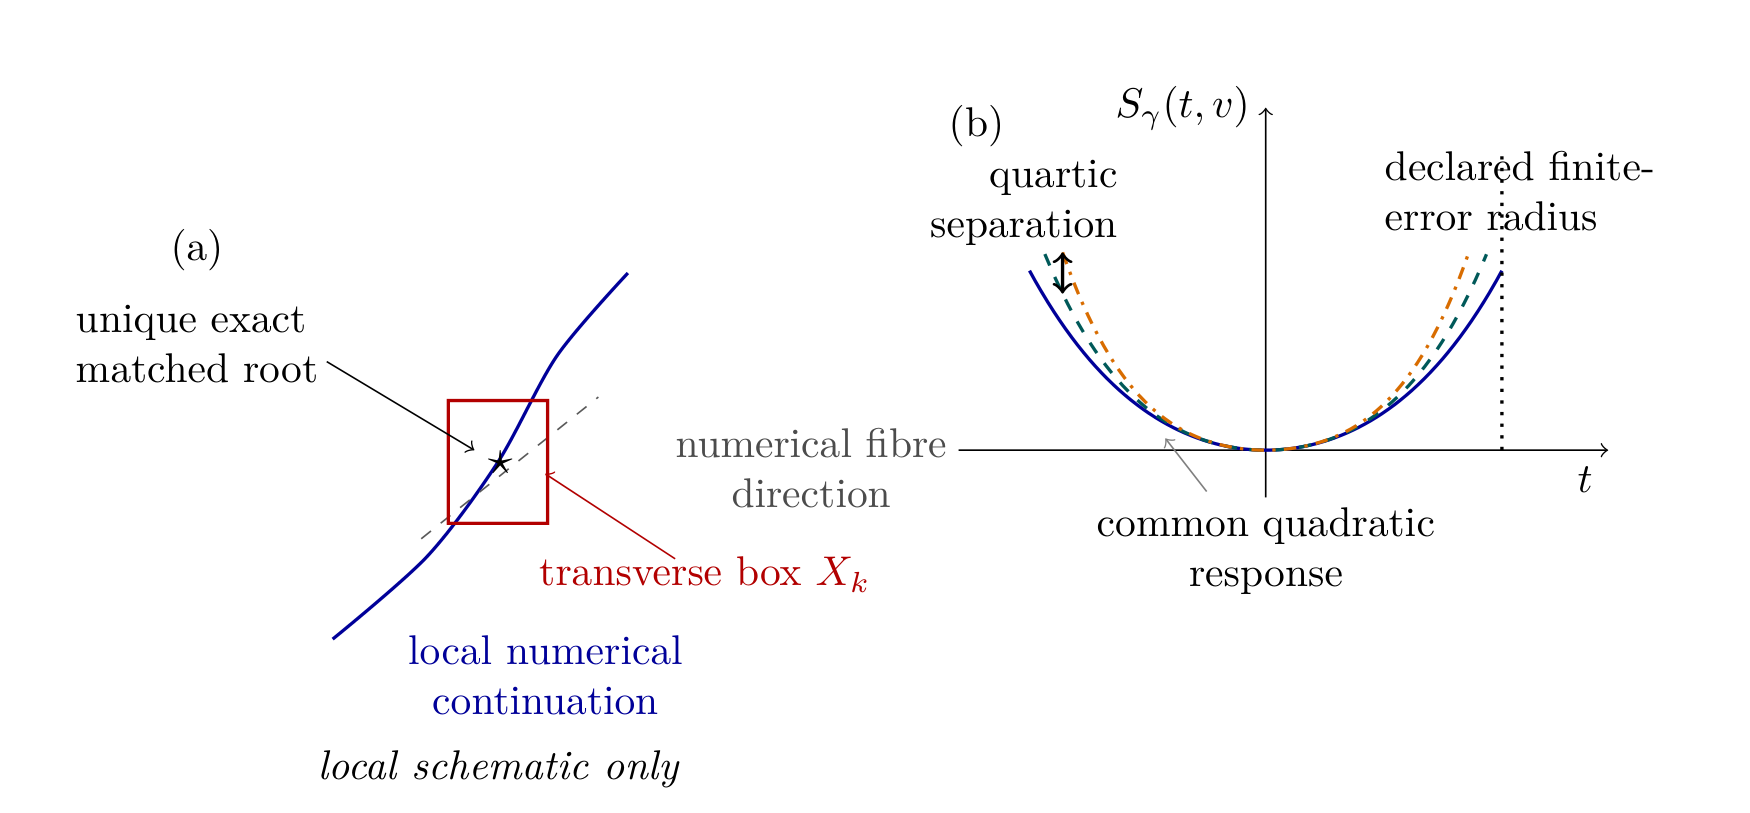
\includegraphics[width=0.9\textwidth]{fig1.png}
\caption{Schematic of local response matching and quartic separation. (a) In a local
control-space chart, the projective output-state and first-response constraints define
numerical tangent directions; the formal certificate establishes a unique exact matched
root only inside each declared transverse box and does not assert a global connected fibre.
(b) Exact projective first-response matching makes the quadratic loss form common.
Symmetrized finite-error responses can therefore first separate through their quartic
coefficients. The tensor $\Aa^{(4)}$ is a fourth-order response susceptibility, not a
Riemannian curvature tensor.}
\label{fig:schematic}
\end{figure}


\section{Prospective fourth-order response prediction}\label{sec:quartic}

\subsection{Symmetric local response}

Introduce normalized error coordinates $z\in\Rr^{3}$ through
\[
\eps=Dz,\qquad D=\diag(0.06,0.04,0.05).
\]
For a direction $v\in\Rr^{3}$, define the symmetric response
\begin{equation}\label{eq:symmetric}
S_{\gamma}(t,v)=\frac{\Iloc_{\gamma}(tDv)+\Iloc_{\gamma}(-tDv)}{2}.
\end{equation}
Analyticity of the finite matrix exponential gives
\begin{equation}\label{eq:taylor}
S_{\gamma}(t,v)=q_{2,\gamma}(v)t^{2}+q_{4,\gamma}(v)t^{4}+q_{6,\gamma}(v)t^{6}+\cdots.
\end{equation}
Odd powers cancel by construction.

By Lemma~\ref{lem:quadratic}, exact projective first-response matching forces the quadratic
loss forms of matched controls to coincide exactly, so the quartic term is the first
possible symmetric discriminator. The numerical cohorts here are matched only within
tolerance; consistently, the relative spread of the averaged quadratic coefficient across
the validation cohorts is approximately $10^{-7}$. The first useful discriminator is
therefore the quartic coefficient.

\subsection{Prospective quartic ranking}

The quartic rule developed here is a \emph{geometric predictor}, not a universal theorem:
it is gap-dependent and certifies only a subset of pairwise comparisons, a boundary made
precise in Sections~\ref{sec:covariant}--\ref{sec:certification}.

\subsubsection{Discovery and validation separation}

The initial four named controls were used only for discovery and orientation. A twelve-path
cohort was then used to compare candidate formulas. The smallest sufficient rule on that
training cohort was
\[
\text{smaller }\Gg_{4}\ \Longrightarrow\ \text{smaller mean finite-error infidelity.}
\]
The addition of the sixth-order coefficient did not improve the training rank correlation,
so the quartic rule was frozen.

For the prospective audit, the coefficients $q_{2},q_{4},q_{6}$ were estimated by a frozen
least-squares fit of
\[
S_{\gamma}(t,e_{a})=q_{2,a}t^{2}+q_{4,a}t^{4}+q_{6,a}t^{6}
\]
at
\[
t\in\Bigl\{\tfrac{1}{32},\tfrac{1}{24},\tfrac{1}{20},\tfrac{1}{16},
\tfrac{1}{14},\tfrac{1}{12},\tfrac{1}{10},\tfrac{1}{8}\Bigr\}.
\]
The tensor audit below is computationally distinct: its directional derivatives are
evaluated directly at $t=0$ by block-matrix exponentials, rather than by fitting
nonzero-radius samples.

A new twenty-path cohort was generated with a different seed. For each candidate, a ranking
certificate containing phases, local coefficients, and predicted order was written and
SHA-256 hashed before the held-out outcome evaluator was enabled. The predeclared primary
gate was
\[
\rho_{\mathrm{Spearman}}\ge 0.95,
\]
together with top-path agreement within each recorded execution.

\subsubsection{Quartic validation result}

The prospective validation result is therefore reported at the predeclared threshold level:
\begin{equation}\label{eq:spearman}
\rho_{\mathrm{Spearman}}\bigl(-\Gg_{4},-\II\bigr)\ge0.95.
\end{equation}
Across the recorded architecture-specific executions ($n=2$) of the prospective
cohort-generation-and-evaluation protocol, the predeclared rank gate was satisfied. The
arm64 reference environment recorded $\rho=0.99398$ with top path pv17, and the
x86\_64/Rosetta diagnostic environment recorded $\rho=0.98947$ with top path pv02; thus the
exact correlation, complete ranking, and named top path were not architecture-invariant,
while both environments cleared the $\rho\ge0.95$ gate. This empirical evidence is not
used in the proof of the exact-root ordering theorem and does not establish a universal
fourth-order ranking law. Because the quartic rule, ranking direction, acceptance threshold,
and ranking certificate were frozen before held-out finite-error evaluation, the
threshold-level result is not an in-sample fit; nevertheless, it remains cohort-specific
prospective evidence rather than a theorem. Two local coefficient-extraction windows had
rank correlation one, and the maximum relative fit residual was $2.37\times10^{-10}$, the
direction-safe upward rendering of the frozen field
\texttt{maximum\_relative\_fit\_residual} in \texttt{results/g4\_prospective/report.json}.

Subsequent cohorts show that $\Gg_{4}$ is not universally sufficient: depending on the
generated matched paths, the prospective quartic correlation varies appreciably across
seeded cohorts. This variation motivated the bounded higher-order analysis rather than post
hoc replacement of the quartic formula.

\section{Covariant quartic response geometry}\label{sec:covariant}

\subsection{Quartic tensor}

The object recovered in this section is a quartic susceptibility of the endpoint loss---a
component of the fourth jet of the endpoint map composed with infidelity---not a
Riemannian curvature or an instance of the quantum geometric tensor~\cite{provost1980}.
There exists a symmetric fourth-order tensor $\Aa^{(4)}_{\gamma}$ such that
\begin{equation}\label{eq:quartictensor}
q_{4,\gamma}(v)=\Aa^{(4)}_{\gamma,ijkl}\,v_{i}v_{j}v_{k}v_{l}.
\end{equation}
In three dimensions a symmetric fourth-order tensor has $\binom{3+4-1}{4}=15$ independent
components. The tensor $\Aa^{(4)}_{\gamma}$ is reconstructed from the fourth jet of the
path-local loss $\Iloc_{\gamma}$: we recover its components from 36 seeded directions,
whose directional Taylor coefficients are computed directly at $t=0$ through order six by
block-matrix exponentials, rather than by fitting nonzero-radius samples.

Let
\[
z\sim\mathrm{Unif}\{\pm e_{\Omega},\pm e_{\Delta},\pm e_{V}\},\qquad \eps=Dz,
\]
so that the physical error scales $0.06^{4},0.04^{4},0.05^{4}$ are carried by $D$ and
absorbed into the tensor components. For the six-axis law in Eq.~\eqref{eq:errorlaw},
define the fourth moment
\[
M^{(4)}_{ijkl}=\ev{z_{i}z_{j}z_{k}z_{l}}.
\]
The scalar quartic predictor is
\begin{equation}\label{eq:g4}
\Gg_{4}(\gamma;M^{(4)})=\Aa^{(4)}_{\gamma,ijkl}M^{(4)}_{ijkl}.
\end{equation}
For the equally weighted signed axes,
\[
\Gg_{4}=\frac{1}{3}\Bigl(\Aa^{(4)}_{\Omega\Omega\Omega\Omega}
+\Aa^{(4)}_{\Delta\Delta\Delta\Delta}+\Aa^{(4)}_{VVVV}\Bigr).
\]

\subsection{Coordinate covariance}

\begin{proposition}[Covariance and invariant contraction]\label{prop:covariance}
Let $z=Ry$ for an invertible real matrix $R$. Then
\begin{equation}\label{eq:atransform}
\Aa^{(4)}_{y,abcd}=\Aa^{(4)}_{z,ijkl}\,R_{ia}R_{jb}R_{kc}R_{ld},
\end{equation}
\begin{equation}\label{eq:mtransform}
M^{(4)}_{y,abcd}=(R^{-1})_{ai}(R^{-1})_{bj}(R^{-1})_{ck}(R^{-1})_{dl}\,M^{(4)}_{z,ijkl},
\end{equation}
and
\begin{equation}\label{eq:invariant}
\Aa^{(4)}_{y}:M^{(4)}_{y}=\Aa^{(4)}_{z}:M^{(4)}_{z}.
\end{equation}
\end{proposition}

\begin{proof}
Equation~\eqref{eq:atransform} follows by substituting $z=Ry$ into the quartic form.
Equation~\eqref{eq:mtransform} follows from $y=R^{-1}z$. Contracting all four indices
cancels each $R$ with the corresponding $R^{-1}$, proving Eq.~\eqref{eq:invariant}.
\end{proof}

This proposition is algebraic. The numerical audit additionally recomputes the tensor
directly in the transformed coordinates. For a nonorthogonal map of condition number
approximately $1.82$, the direct-refit relative error is $1.08\times10^{-14}$ and the
maximum invariant-contraction relative error is $2.36\times10^{-15}$.

The covariant object is not the scalar $\Gg_{4}$ in isolation. It is the fourth-order
response tensor $\Aa^{(4)}$ together with the physical fourth noise moment $M^{(4)}$. Their
contraction is independent of a linear reparameterization of error coordinates. This avoids
interpreting a coordinate-specific axis average as an intrinsic curvature.

Establishing a relation of this susceptibility to a canonical connection or curvature on a
control quotient would require additional structure.

For a noise moment $M$, the low-cost screening problem is
\[
\gamma^{\star}\in\argmin_{\gamma\in\Ff_{\eta_{\mathrm{match}}}}\ \Aa^{(4)}_{\gamma}:M^{(4)}.
\]
Pairs that fail the quartic gap test can be escalated adaptively to sixth, eighth, or
higher jet order until their intervals separate. This suggests a certified branch-and-bound
control selector: compute low-order local tensors for all candidates, refine only ambiguous
pairs, and reserve direct finite-error simulation or hardware evaluation for model
validation rather than exhaustive ranking.

The gap-dependent certification criterion used by the implementation retains the residual
constant and quadratic terms explicitly. The certified quantity is the six-axis averaged
reference loss at radius $t$,
\begin{equation}\label{eq:radiusloss}
\Iref_{k}(t)=\frac{1}{6}\sum_{a\in\{\Omega,\Delta,V\}}\sum_{\sigma=\pm1}
\Iref_{k}(\sigma t D e_{a}).
\end{equation}
At unit radius $t=1$ the six signed probe points $\sigma D e_{a}$ are exactly the six
signed axial errors of the declared error set, so Eq.~\eqref{eq:radiusloss} reduces to the
six-axis mean functional of Eq.~\eqref{eq:meanloss}; the radius-$t$ form is its
one-parameter rescaling used for the local jet analysis.
For each path $k$ write the truncated local model and its enclosure as
\begin{equation}\label{eq:truncated}
P_{k}(t)=C_{0,k}+C_{2,k}t^{2}+\Gg_{4,k}t^{4},\qquad
\Iref_{k}(t)\in P_{k}(t)+[-B_{k}(t),\,B_{k}(t)].
\end{equation}
If
\begin{equation}\label{eq:gaptest}
\lvert P_{a}(t)-P_{b}(t)\rvert > B_{a}(t)+B_{b}(t),
\end{equation}
then the sign of $\Iref_{a}(t)-\Iref_{b}(t)$ is strictly certified. Only when
$C_{0,a}=C_{0,b}$ and $C_{2,a}=C_{2,b}$ does this reduce to the simplified quartic-gap form
\[
\lvert\Gg_{4,a}-\Gg_{4,b}\rvert\,\lvert t\rvert^{4} > B_{a}(t)+B_{b}(t).
\]
The implementation folds the residual $C_{0}$ and $C_{2}$ differences into the correction
intervals, so they are not omitted from the certificate.

\section{Computer-assisted certification}\label{sec:certification}

\subsection{Krawczyk root theorem}

The numerical paths satisfy the endpoint and first-order matching constraints to order
$10^{-11}$ (see Remark~\ref{rem:residual} for the precise norm and its relation to the
formal boxes). To move from numerical candidates to exact mathematical roots, we use the
projective constraint map $F:\Rr^{24}\to\Rr^{16}$ of Eq.~\eqref{eq:constraintmap}. We do
\emph{not} split the 24 original phase coordinates into a fixed subset of 16 transverse
coordinates and 8 retained fibre coordinates. Instead, for each frozen path $k$ the
certificate uses the affine transverse parameterization
\begin{equation}\label{eq:affine}
\gamma=\widehat{\gamma}_{k}+N_{k}\,x,
\qquad x\in X=[-3\times10^{-12},\,3\times10^{-12}]^{16}\subset\Rr^{16},
\end{equation}
where $\widehat{\gamma}_{k}\in\Rr^{24}$ is the frozen box centre of path $k$ and the
columns of the frozen $24\times16$ matrix $N_{k}$ form the declared orthonormal transverse
basis. The variable $x$ is the vector of transverse-basis coefficients, not a selection of
16 of the original 24 phase coordinates, and $N_{k}$ varies from path to path. On this
declared affine transverse slice we consider the reduced square map
\[
F_{k}(x)=F(\widehat{\gamma}_{k}+N_{k}x),\qquad F_{k}:\Rr^{16}\to\Rr^{16},
\]
whose Jacobian is the reduced $16\times16$ matrix
\begin{equation}\label{eq:reducedjac}
DF_{k}(x)=DF(\widehat{\gamma}_{k}+N_{k}x)\,N_{k}\in\Rr^{16\times16}.
\end{equation}
All interval operators below act on this path-dependent reduced map; at no point is a
transverse vector $x\in\Rr^{16}$ passed directly to $F:\Rr^{24}\to\Rr^{16}$. For a box
$X\subset\Rr^{16}$ with centre $x_{0}$, the Krawczyk operator for path $k$ is
\begin{equation}\label{eq:krawczyk}
K_{k}(X)=x_{0}-C_{k}F_{k}(x_{0})+\bigl(I-C_{k}[DF_{k}(X)]\bigr)(X-x_{0}),
\end{equation}
where $C_{k}$ is the frozen point preconditioner of the corresponding reduced midpoint
Jacobian $DF_{k}(x_{0})$ (a numerical approximate inverse) and $[DF_{k}(X)]$ is an
interval enclosure of the reduced Jacobian~\eqref{eq:reducedjac} over $X$. In centered
coordinates $x_{0}=0$, as used by the implementation, this reduces to
\[
K_{k}(X)=-C_{k}F_{k}(0)+\bigl(I-C_{k}[DF_{k}(X)]\bigr)X.
\]
The strict inclusion $K_{k}(X)\subset\intt(X)$ then implies that $F_{k}$ has a unique
zero inside $X$~\cite{moore2009,tucker2011}. The projective chart denominator $\psi_{0}$ of
Eq.~\eqref{eq:chart} is formally verified to exclude zero on every accepted box, ensuring
the coordinate chart is valid throughout the Krawczyk computation.

\begin{theorem}[Krawczyk inclusions for 12 declared controls]\label{thm:krawczyk}
For each of the twelve declared controls, with the affine transverse parameterization of
Eq.~\eqref{eq:affine}, the common transverse box
\[
X_{k}=X=[-3\times10^{-12},\,3\times10^{-12}]^{16}
\]
satisfies the strict Krawczyk inclusion
\[
K_{k}(X_{k})\subset\intt(X_{k}).
\]
Consequently, each box $X_{k}$ contains a unique exact root $x^{\ast}_{k}$ of
$F_{k}(x)=0$, i.e., a control
$\gamma^{\ast}_{k}=\widehat{\gamma}_{k}+N_{k}x^{\ast}_{k}$ that is exactly matched in
projective output state and first projective response to the reference. Existence and
uniqueness are certified within the declared transverse box only, not on the full
24-dimensional phase space or the whole response fibre.
\end{theorem}

\begin{proof}[Computer-assisted proof]
A numerical approximate inverse of the midpoint Jacobian is used as the point
preconditioner. The Jacobian over each full box is then enclosed with 192-bit Arb
arithmetic, and the resulting Krawczyk image is verified to lie strictly inside the box.
The projective chart denominator is formally verified to exclude zero on every accepted
box. For all twelve boxes, the inclusion $K_{k}(X)\subset\intt(X)$ is verified; the worst
box-normalized utilization, read from the frozen certificate, is
\[
\max_{k}\frac{\lVert K_{k}(X)\rVert_{\infty}}{3\times10^{-12}}<0.866<1,
\]
so every coordinate image clears the box wall by a factor of at least $1.15$. The SHA-256
protocol and certificate identifiers of this run are recorded in
Appendix~\ref{app:hashes}. By the Krawczyk
theorem~\cite{moore2009,tucker2011,tucker2002}, each box contains a locally unique root.
As a \emph{supplementary} audit-closure check---not an additional premise of the strict
inclusion just established---the regularity of each frozen point preconditioner is
independently certified by a $256$-bit outward-rounded Rump--Neumann argument: for all
twelve paths $\lVert I-R_{k}C_{k}\rVert_{\infty}<1$, so each $C_{k}$ is nonsingular
(certificate \nolinkurl{results/audit_closure/p0_preconditioner_certificate.json}). This
P0 certificate belongs to the later v0.3.2 audit-closure supplement
(Remark~\ref{rem:p0role}); it strengthens auditability but neither replaces nor alters the
v0.3.1 frozen Krawczyk certificate that proves the theorem. In the strict-inclusion form
of the Krawczyk theorem used here, the required regularity is already implied by the
accepted inclusion; the v0.3.2 P0 certificate is therefore an independent redundant audit
of the production preconditioner, not an additional premise of Theorem~\ref{thm:krawczyk}.
\end{proof}

\begin{remark}[Residual, norm, and box relation]\label{rem:residual}
Two distinct residuals must not be conflated. The \emph{unpreconditioned} constraint
residual $\lVert F\rVert$ of the numerical candidates is of order $10^{-11}$; it is a
float64 diagnostic of the candidate-generation optimizer and is \emph{not} compared
directly with the $3\times10^{-12}$ box radius. The strict Krawczyk inclusion is decided
instead by the full interval image
$-C_{k}F_{k}(x_{0})+\bigl(I-C_{k}\,[DF_{k}(X)]\bigr)(X-x_{0})$
of Eq.~\eqref{eq:krawczyk}, whose outward-rounded endpoints are enclosed on the formal
cohort box centres $\widehat{\gamma}_{k}$. The preconditioned image
$\lVert K_{k}(X)\rVert_{\infty}$, already preconditioned by $C_{k}$, is what the
utilization bound $0.866$ above reports. The frozen certificate does not tabulate a single
scalar preconditioned centre residual; accordingly we do not quote one, and the
$10^{-11}$ figure refers only to the unpreconditioned optimizer residual.
\end{remark}

\begin{remark}[Scope of the Krawczyk inclusion theorem]
The theorem establishes local uniqueness inside each declared transverse box. It does not
certify global uniqueness on the entire fibre, nor does it prove that every point on the
numerical fibre has an exact representative. The global fibre structure remains open.
\end{remark}

\subsection{Direct finite-error ordering theorem}

The following theorem is the main result of this work. Its proof uses only the certified
Krawczyk boxes and direct outward-rounded propagation of the finite-error functional. No
Taylor truncation, Cauchy extraction, alias enclosure, or local-jet reconstruction is used.

\begin{theorem}[Exact-root finite-error ordering]\label{thm:ordering}
For each of the twelve declared controls, let $X_{k}$ be the transverse phase box
satisfying a strict Krawczyk inclusion from Theorem~\ref{thm:krawczyk}. Direct
outward-rounded Arb propagation of $X_{k}$ through the declared six-point finite-error
functional produces twelve performance intervals $B_{k}$ covering the complete root box,
\[
B_{k}\supseteq
\Bigl\{\,\overline{\mathcal{E}}\bigl(\widehat{\gamma}_{k}+N_{k}x\bigr):
x\in[-3\times10^{-12},\,3\times10^{-12}]^{16}\Bigr\},
\]
that are pairwise disjoint and totally
ordered according to the pre-outcome ordering frozen for the independent twelve-path
formal cohort. Therefore the locally
unique roots exactly matched in projective output state and first projective response
inside the boxes obey the complete frozen finite-error ordering.
\end{theorem}

\begin{proof}[Computer-assisted proof]
By Theorem~\ref{thm:krawczyk}, the locally unique projectively matched control
$\gamma^{\ast}_{k}=\widehat{\gamma}_{k}+N_{k}x^{\ast}_{k}$ belongs to the certified box.
For every box $X_{k}$, the six declared finite-error Hamiltonians are evaluated directly
using 192-bit outward-rounded Arb/ACB arithmetic over the \emph{whole} declared transverse
box, not merely at its centre or at the approximate root: every phase-dependent
trigonometric factor, Hamiltonian matrix exponential, state propagation, overlap,
infidelity, and six-point mean is enclosed. Denote the resulting real performance interval
by $B_{k}$. Because the propagation is over the full box,
\[
B_{k}\supseteq
\Bigl\{\,\overline{\mathcal{E}}\bigl(\widehat{\gamma}_{k}+N_{k}x\bigr):
x\in[-3\times10^{-12},\,3\times10^{-12}]^{16}\Bigr\},
\]
where $\overline{\mathcal{E}}$ is the six-axis mean finite-error functional of
Eq.~\eqref{eq:meanloss}. Since the certified root satisfies $x^{\ast}_{k}\in X$, its
exact-root performance lies in the enclosure,
\[
\II(\gamma^{\ast}_{k})\in B_{k}.
\]
No Taylor truncation, order-30 jet, or local-jet reconstruction enters $B_{k}$. For every
frozen ordered pair $a\prec b$, direct interval comparison verifies
\[
\sup B_{a}<\inf B_{b}.
\]
All $\binom{12}{2}=66$ comparisons pass and have the orientation specified by the frozen
ordering certificate. Because each $B_{k}$ encloses its exact root's performance, the
strict box separation $\sup B_{a}<\inf B_{b}$ implies the strict exact-root ordering
\[
\II(\gamma^{\ast}_{a})<\II(\gamma^{\ast}_{b})
\]
for every frozen ordered pair.
\end{proof}

The predecessor order was frozen before direct propagation; the resulting protocol and
certificate hashes are reported in Appendix~\ref{app:hashes}.

\begin{remark}[Scope of Theorem~\ref{thm:ordering}]
The theorem is conditional on the serialized-decimal finite Hamiltonian model, the declared
transverse boxes, and the six-axis mean error functional. It does not certify model
discrepancy, global fibre topology, many-body scaling, or hardware. It also does not prove
a global eight-dimensional exact fibre theorem; it proves finite-error ordering for the
locally unique exact roots inside the declared boxes.
\end{remark}

\begin{corollary}[Ordering stability under bounded loss discrepancy]\label{cor:stability}
Let $B_{k}$ denote the certified direct performance interval for the $k$th exact root, and
define the minimum certified ordering margin
\[
\Delta_{\min}=\min_{a\prec b}\bigl(\inf B_{b}-\sup B_{a}\bigr)>0,
\]
where $a\prec b$ ranges over the frozen ordered path pairs. Suppose an additional physical
effect changes the evaluated loss of every fixed certified control by at most $\eta$:
\[
\bigl\lvert\widetilde{\II}(\gamma^{\ast}_{k})-\II(\gamma^{\ast}_{k})\bigr\rvert\le\eta
\quad\text{for every }k.
\]
If
\[
2\eta<\Delta_{\min},
\]
then the complete frozen ordering of the twelve fixed certified controls is preserved under
the perturbed loss.
\end{corollary}

\begin{proof}
For every frozen ordered pair $a\prec b$,
\[
\widetilde{\II}(\gamma^{\ast}_{a})\le\sup B_{a}+\eta
<\inf B_{b}-\eta\le\widetilde{\II}(\gamma^{\ast}_{b}),
\]
where the strict middle inequality follows from $2\eta<\Delta_{\min}$.
\end{proof}

For the frozen twelve-root certificate, the minimum formally certified pairwise margin,
computed from the outward-rounded endpoints of the frozen direct-certificate intervals, is
\[
\Delta_{\min}=2.50\times10^{-5},
\]
attained by the pair pv08 and pv11.
For the certified minimum separation $\Delta_{\min}=2.505874\ldots\times10^{-5}$, the
sufficient uniform perturbation condition in Corollary~\ref{cor:stability} becomes
$\eta<\Delta_{\min}/2\approx1.25\times10^{-5}$. This is a stringent model-discrepancy
requirement and should not be interpreted as a certificate of hardware-level ordering
robustness.

Corollary~\ref{cor:stability} is a conditional stability statement for the losses evaluated
at the same certified controls. It does not prove that an added Lindblad term, waveform
filter, calibration drift, or other model perturbation satisfies the required bound, nor
that the controls remain exact response-matched roots of the perturbed model. Proving root
continuation under model perturbation would require a parameterized Krawczyk or validated
implicit-function argument.

\subsection{Order-thirty mechanism certificate}

The following proposition provides a separate, computationally distinct mechanism
certificate using the zero-error jet. Unlike the main theorem, it uses Taylor coefficients,
Cauchy extraction, alias enclosures, and Dyson tail bounds. It is not part of the main
theorem proof.

The floating-point precursor obtains the order-thirty jet by block-matrix exponentials. The
formal phase-box certificate used in Proposition~\ref{prop:order30} instead extracts the
coefficients with a 64-point outward-rounded Cauchy transform.

\begin{proposition}[Order-thirty mechanism certificate]\label{prop:order30}
Propagation of the zero-error jet through order thirty over the twelve Krawczyk phase
boxes, including the formal Cauchy-alias and analytic order-32 tail enclosures, certifies
52/66 frozen path pairs. Every certified orientation agrees with the frozen order, and no
reversed pair is certified.
\end{proposition}

\begin{proof}[Computer-assisted proof]
For path $k$ and physical error axis $a$, define the analytic transition amplitude
\[
g_{k,a}(\lambda)=\braket{\psi_{\mathrm{ref}}}{\psi_{\gamma_{k}}(\lambda De_{a})}
=\sum_{n\ge0}g_{k,a,n}\,\lambda^{n}.
\]
Its coefficients are extracted by a 64-point outward-rounded Cauchy discrete Fourier
transform on the complex unit circle:
\begin{equation}\label{eq:cauchy}
\widehat{g}_{n}=\frac{1}{64}\sum_{k=0}^{63}g(\zeta_{k})\,\zeta_{k}^{-n},
\qquad \zeta_{k}=e^{2\pi i k/64}.
\end{equation}
The discrete transform aliases coefficients $g_{n+64\ell}$. A path-uniform Dyson
bound~\cite{dyson1949} encloses this alias. The implemented enclosure is $10^{-40}$, and the formal gate verifies
that
\[
\frac{e^{K_{a}}K_{a}^{64}}{64!}<10^{-40}
\]
for every physical error axis, where the dependence is parameterized as
\[
H_{a}(s;\lambda_{a})=H_{0}(s)+\lambda_{a}H_{1,a}(s),
\]
with $s$ the physical time and $\lambda_{a}$ the dimensionless error parameter along axis
$a$, and
\[
K_{a}=\int_{0}^{T}\lVert H_{1,a}(s)\rVert_{2}\,ds
=\int_{0}^{T}\left\lVert
\frac{\partial H_{a}(s;\lambda_{a})}{\partial\lambda_{a}}
\bigg|_{\lambda_{a}=0}\right\rVert_{2}ds
\]
is the integrated spectral norm of the Hamiltonian perturbation along axis $a$. Fidelity
coefficients are formed by ball convolution,
\[
F_{n}=\sum_{r=0}^{n}g_{r}\,\bar{g}_{n-r},
\]
and the infidelity coefficients follow from $1-F$. The mean six-axis analytic even Dyson
tail after order thirty is enclosed by $2\times10^{-11}$; the largest individual-axis tail
is below $4\times10^{-11}$.

Propagating the resulting order-thirty jet over the twelve Krawczyk phase boxes yields
performance intervals. Pairwise comparison of the resulting order-thirty intervals
certifies 52/66 frozen path pairs. Every certified orientation agrees with the frozen
order, and no reversed pair is certified. The unresolved pairs arise from dependency and
wrapping in the phase-box propagation of the jet enclosure. They are not reversed physical
comparisons and do not indicate an omitted-tail failure.
\end{proof}


\begin{table}[t]
\centering
\caption{Representative prospective and formal audits. ``Rank diagnostic'' denotes the
Spearman correlation of the corresponding ranking stage; covariance itself is verified by
the $10^{-14}$--$10^{-15}$ relative residuals collected in Appendix~\ref{app:hashes}.
``Certified result'' states the certified object explicitly, distinguishing certified roots
from certified unordered pairs. Candidate sets differ between stages and between numerical
environments; every stage freezes its protocol and ranking before held-out evaluation. The
direct exact-root ordering is the main theorem.}
\label{tab:audits}
\footnotesize
\begin{tabular}{@{}lllll@{}}
\toprule
Audit & Paths & Rank diagnostic & Certified result & Logical role\\
\midrule
Prospective $\Gg_{4}$ ranking & 20 & $\rho=0.996992$ & -- & prospective evidence\\
Covariant $\Gg_{4}$ contraction ranking & 12 & $\rho=0.965035$ & -- & covariance/ranking audit\\
Formal quartic-only bound & 12 & -- & 34/66 pairs & low-order boundary\\
Frozen numerical-point order-30 & 12 & $\rho=1$ & 66/66 pairs & diagnostic\\
Exact-root Krawczyk inclusion & 12 & -- & 12/12 roots & existence/uniqueness\\
Exact-root order-30 jet & 12 & -- & 52/66 pairs & mechanism certificate\\
Exact-root direct Arb propagation & 12 & $\rho=1$ & 66/66 pairs & main theorem\\
\bottomrule
\end{tabular}
\end{table}

\section{Results}\label{sec:results}

\textbf{Frozen-point diagnostic.} For the twelve serialized numerical phase points, before
propagation over the Krawczyk root boxes, the order-thirty jet and its analytic tail
enclosure certify all 66/66 pairwise comparisons. This pointwise diagnostic is witnessed by
the proof objects in \texttt{results/l4\_order30/}. It is not an exact-response-root
certificate. Propagation over the certified root boxes subsequently resolves 52/66 pairs
with zero reversals (Proposition~\ref{prop:order30}).

Numerical integrity diagnostics from representative runs are collected in
Appendix~\ref{app:hashes}. The sequence of results supports the following hierarchy.
\begin{enumerate}[itemsep=0.1em]
\item \textbf{Implementation memory:} endpoint and complete first-order output-state
matching do not numerically determine finite-error performance.
\item \textbf{Low-order organization:} the covariant quartic contraction $\Gg_{4}$ strongly
organizes mean performance and formally certifies a substantial subset of path pairs
(34/66 at the formal ball level).
\item \textbf{Exact-root certification:} strict Krawczyk inclusions establish 12 locally
unique roots exactly matched in projective output state and first projective response.
\item \textbf{High-order mechanism:} the order-thirty jet propagated over the Krawczyk
boxes certifies 52/66 pairs with zero reversals (Proposition~\ref{prop:order30}).
\item \textbf{Complete ordering:} direct 192-bit outward-rounded Arb propagation of the
Krawczyk boxes certifies all 66 pairs with the frozen order preserved
(Theorem~\ref{thm:ordering}).
\end{enumerate}

Figure~\ref{fig:evidence} displays the two data-level statements behind the title: the
prospective ranking on the held-out cohort and the certified exact-root intervals of the
main theorem.

\begin{figure}[t]
\centering
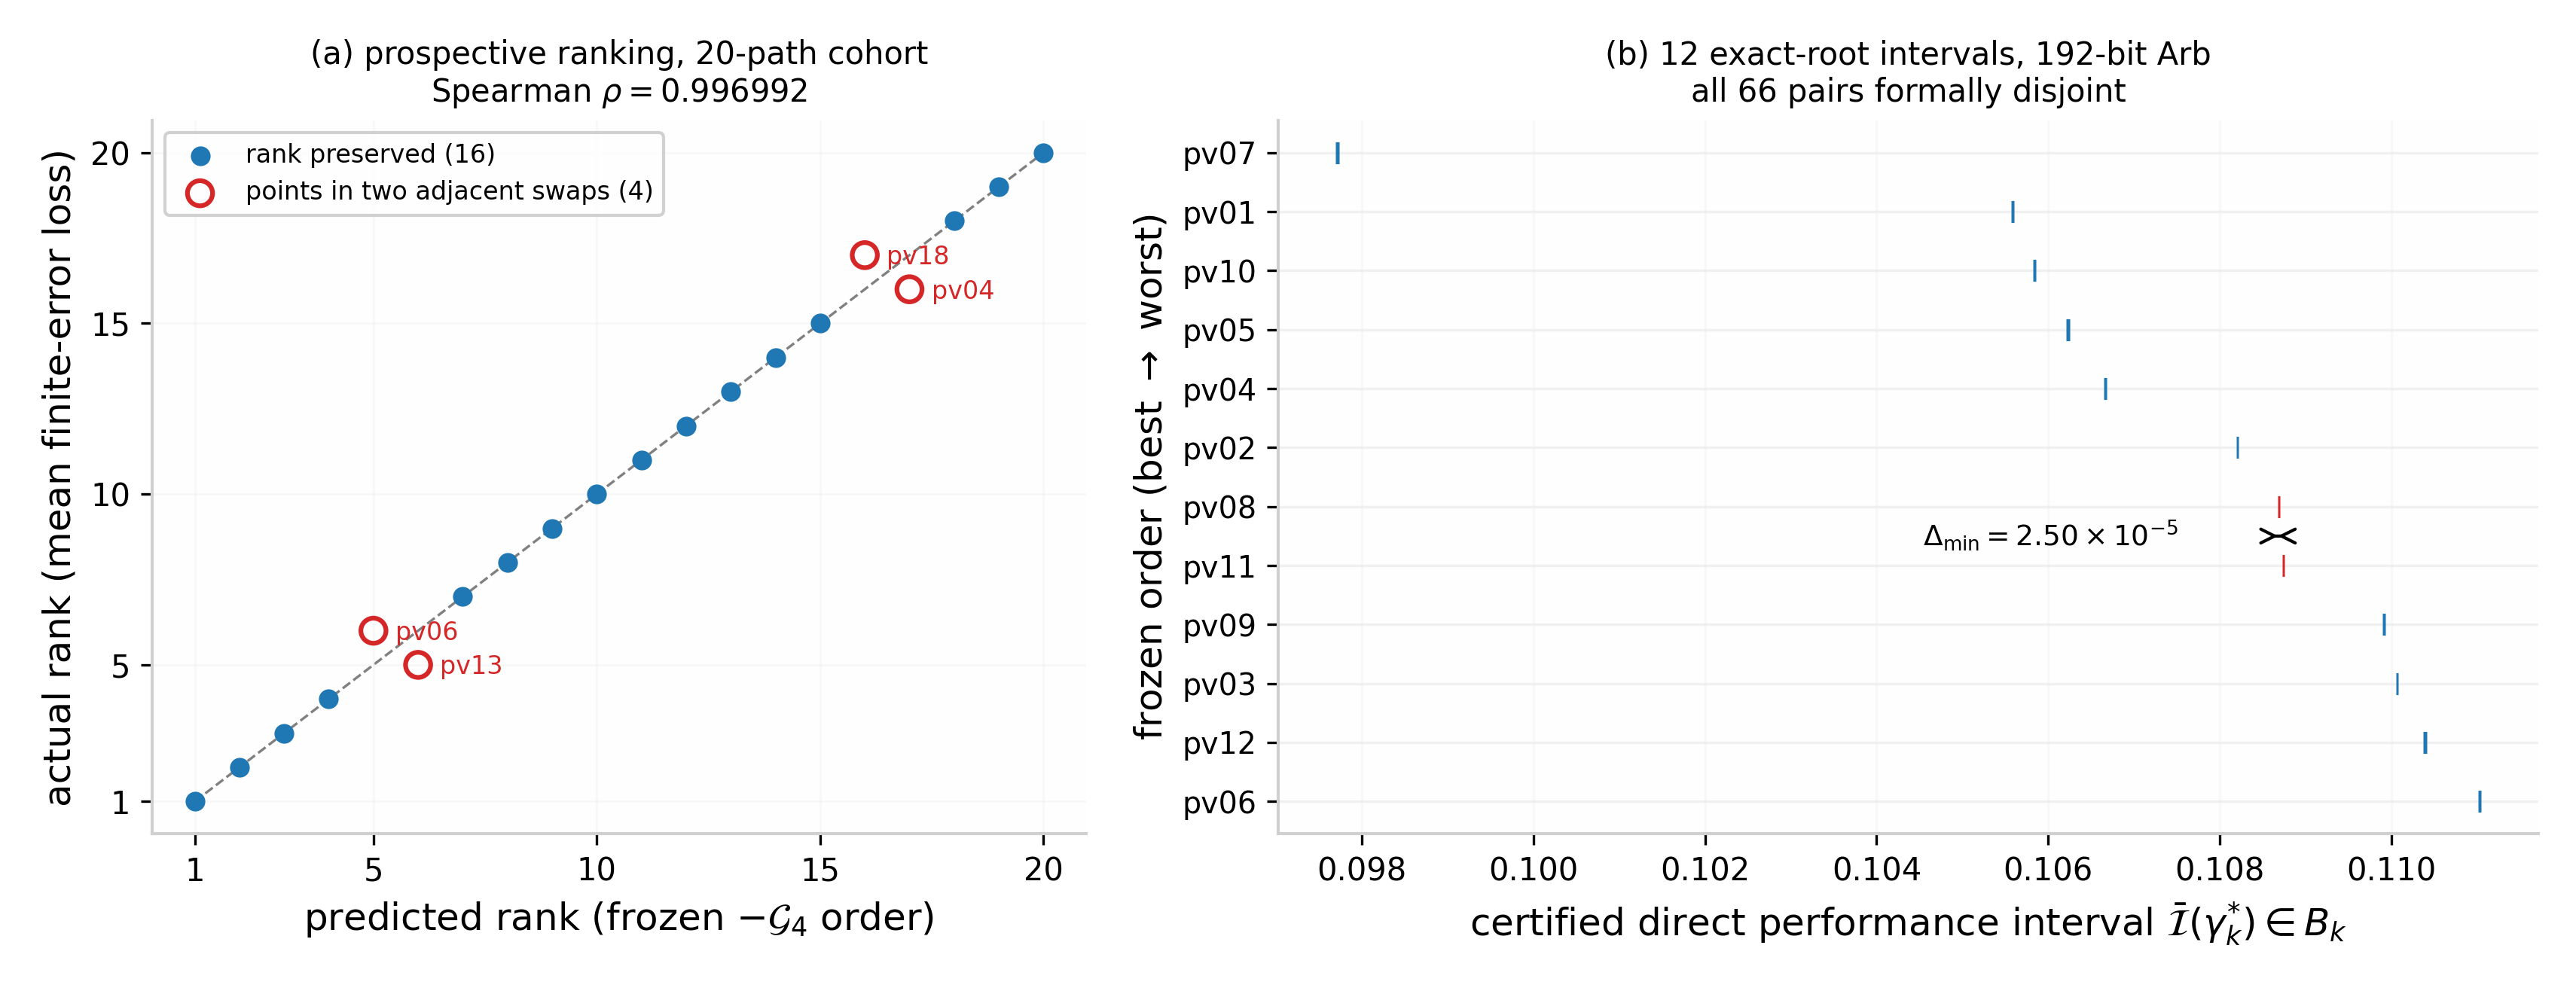
\includegraphics[width=0.95\textwidth]{fig2.png}
\caption{Direct visual evidence for the two claims in the title. (a) Prospective
prediction: $-\Gg_{4}$ predicted versus actual ranks on the held-out twenty-path cohort.
The frozen order reproduces the actual mean-loss ranking up to two adjacent transpositions
(marked), giving Spearman $\rho=0.996992$. This panel reports prospective empirical
evidence; it is not a certificate. (b) Exact-root certification: the twelve certified
direct performance intervals $B_{k}$ from 192-bit outward-rounded Arb propagation, drawn to
scale in the frozen order. All 66 unordered pairs are formally disjoint; the tightest pair,
pv08--pv11, has the certified margin $\Delta_{\min}=2.50\times10^{-5}$ of
Corollary~\ref{cor:stability} (inset: magnification of that pair).}
\label{fig:evidence}
\end{figure}

\section{Discussion}\label{sec:discussion}

\subsection{Why the quartic term is useful but incomplete}

First-order matching makes the quadratic loss nearly common---exactly common at exact
matched roots by Lemma~\ref{lem:quadratic}. This promotes the quartic term to the first
visible discriminator. It explains why $\Gg_{4}$ often gives almost perfect rankings.
However, if two quartic coefficients are close, the sixth and higher terms can reverse
their order. The formal intervals expose this distinction directly: 34 pairs are
quartic-certified, while the remaining pairs require higher jet data or direct propagation.

This is preferable to declaring the quartic rule either universally true or false. The
correct statement is gap-dependent as in Eq.~\eqref{eq:gaptest}.

\subsection{Minimal model versus scalable certification}

The role of the two-atom model is to isolate the response-matching mechanism in the
smallest interacting Rydberg system, not to approximate a many-body processor. The present
certificate shows that residual finite-error ordering survives exact projective state and
complete first-response matching without being attributable to optimizer residuals. Turning
this result into a many-body compilation method requires a separate scalability programme,
including structured state representations and dependency-preserving validated propagation.
The current theorem should therefore be read as a minimal rigorous existence-and-ordering
result rather than as a scalable hardware-design algorithm.

\subsection{Order-30 mechanism versus direct propagation}

The order-30 jet propagated over the Krawczyk boxes certifies 52/66 pairs with zero
reversals (Proposition~\ref{prop:order30}). The remaining 14 pairs are not physically
reversed---they are unresolved due to dependency and wrapping in the phase-box propagation
of the jet enclosure. Direct Arb propagation of the same boxes certifies all 66 pairs
(Theorem~\ref{thm:ordering}), demonstrating that the unresolved cases are an artefact of
the jet propagation and interval wrapping, not a physical failure of the frozen ordering.
The 52/66 mechanism certificate and the 66/66 direct certificate arise from different
propagation levels and should not be conflated: the latter is the main theorem.

The content is quantitative rather than existential: an analytic finite-dimensional
propagator is determined by its local germ, but here a fixed finite order, 30, resolves
52/66 comparisons with an explicitly bounded tail, and the unresolved cases arise from
interval wrapping rather than truncation.

The particular ordering of the twelve serialized controls is not presented as a universal
physical law. The reusable contribution is the certificate architecture: transverse
exact-root isolation, formal propagation of the resulting root boxes, and explicit
separation between low-order mechanism certificates and direct finite-error theorems.

\section{Limitations and next theorem}\label{sec:limitations}

The present work has five explicit limitations.
\begin{enumerate}[itemsep=0.15em]
\item \textbf{Global fibre structure.} Twelve locally unique roots exactly matched in
projective output state and first projective response are certified in transverse boxes.
The global eight-dimensional solution manifold structure remains unproved.
\item \textbf{Finite-dimensional model.} Spontaneous emission, Doppler effects, laser phase
noise, position fluctuations, leakage levels, and waveform filtering are absent. An
open-system extension is not obtained by appending a dissipative curve to the present
certificate. Exact matching of density matrices or quantum channels and their first
responses defines a different constraint map, whose dimension generally scales with
$d^{2}$ rather than $d$. It would require new matched controls, new root boxes, and
validated Liouvillian propagation. Arbitrary dissipative perturbations need not preserve
the present ordering, and no noise-model-independent ordering theorem is claimed here.
\item \textbf{Two atoms.} No many-body scaling theorem is claimed.
\item \textbf{Mean axial error law.} The primary result concerns the declared six-axis
mean. Worst-case ranking is not supported by the present scalar.
\item \textbf{No QPU evidence.} The calculations are local and require no hardware access.
They do not constitute physical-QPU evidence.
\end{enumerate}
In short, the certificate is formal for the serialized finite-dimensional two-atom
Hamiltonian, the declared transverse boxes, and the six-axis mean error functional; it does
not certify model discrepancy, global fibre topology, many-body scaling, or hardware.

\subsection{Constraint dimension and scalability}

The present dense interval implementation is not a scalable many-body compiler. Its
dimensional growth can nevertheless be stated explicitly. Suppose the reachable complex
state space has dimension $d$, and let $m$ be the number of calibrated error coordinates.
Matching one projective output state and its $m$ complete projective first responses
imposes
\[
q=2(m+1)(d-1)
\]
real projective constraints. When the constraint Jacobian has rank $q$, a square Krawczyk
chart uses $q$ transverse control variables, while any remaining independent control
variables parameterize numerical fibre directions.

Here $m=3$ and the exchange-symmetric two-atom state space has $d=3$, giving
\[
q=2(3+1)(3-1)=16,
\]
with $24-16=8$ numerical fibre directions. For a fully permutation-symmetric $N$-atom
two-level model, $d=N+1$ and the corresponding constraint count is $8N$. For a generic
unsymmetrized model, $d=2^{N}$ and the dense constraint count becomes $8(2^{N}-1)$.

Thus exponential growth is not intrinsic to the Krawczyk operator alone; it arises through
the dimension of the reachable state representation and the cost of enclosing the
associated propagators and Jacobians. In generic many-body settings, direct dense Arb/ACB
propagation and naive interval Jacobians would also suffer rapidly increasing dependency
and wrapping. Possible routes to larger systems include symmetry reduction, sparse or
block-structured propagation, reduced-observable matching, tensor-network enclosures,
Taylor or Chebyshev polynomial models with validated remainder bounds, interval
subdivision, and parameter-dependent Krawczyk charts. Taylor or Chebyshev polynomial models
with validated remainder bounds may help reduce local propagation overestimation, but they
do not by themselves remove the exponential growth of a generic many-body state
representation. None of these extensions is implemented or certified in the present work.

The next mathematical step is a validated implicit-function theorem or a
parameter-dependent Krawczyk atlas: treat the eight fibre coordinates as parameters and
certify a unique transverse solution varying over a declared fibre neighbourhood. The
target mathematical structure is
\[
F(x,y)=0,\qquad x\in\Rr^{16},\ y\in\Rr^{8},
\]
and the goal is to prove that a unique transverse solution $x=x(y)$ exists and is regular
over a declared $y$-region, not to prove a single global isolated root.

\section{Reproducibility}\label{sec:repro}

The complete formal pipeline is frozen in a single standalone audit (v1.3). The
twelve-path cohort, the transverse bases, and the point preconditioners are fixed; the
common Krawczyk radius is $3\times10^{-12}$; and runtime metadata is excluded from every
hashed proof object. Two complete formal executions produce byte-identical protocol,
certificate, and report files. The SHA-256 certificate identifiers and the numerical
integrity diagnostics are collected in Appendix~\ref{app:hashes}; the script inventory,
dependency pins, and clean-environment runs are collected in Appendix~\ref{app:scripts}.

\textbf{Clean-environment reproduction.} The complete v1.3 audit was rerun in a clean
external Colab environment from the public v0.3.1 Git tag, which resolved to commit
\begin{center}
\footnotesize\texttt{284974c9f6b952f4e114c8c5bdc9c2c299c4065c}.
\end{center}
Dependency installation, repository
SHA-256 verification, reference-artifact validation, regression tests, and the complete
two-run formal recomputation all passed. The run required no vendor account or cloud
credentials.

\section{Conclusion}\label{sec:conclusion}

We establish two complementary results on distinct frozen cohorts. On a prospective
twenty-path cohort, the zero-point quartic geometric scalar strongly predicts held-out
finite-error performance. On a separate twelve-path formal cohort, direct outward-rounded
interval propagation certifies all 66 pairwise finite-error orderings at locally unique
roots exactly matched in projective output state and first projective response.

The common endpoint and complete first-order state response leave residual path dependence.
A coordinate-covariant fourth-order response tensor provides a strong and partially
certifying low-order description, but close comparisons require higher derivatives. On the
twelve-path cohort, strict Krawczyk inclusions establish the twelve locally unique exact
roots. The zero-error jet through order thirty, combined with rigorous Cauchy-alias and
Dyson-tail enclosures, certifies 52/66 exact-root comparisons with zero reversals as a
separate mechanism certificate. Direct 192-bit outward-rounded Arb propagation of the
Krawczyk boxes certifies all 66 pairwise orderings as the main theorem.

The explicit constraint-dimension count identifies the boundary of the present dense
certificate: it remains tractable in the minimal interacting model and in suitably reduced
symmetry sectors, but no generic many-body scalability claim is made. The next steps are
parameterized root continuation, certified model-discrepancy budgets, structured many-body
propagation, and separate open-system and compiled-hardware validation.

\appendix

\section{Interval-arithmetic certificate construction}\label{app:interval}

For completeness we collect the construction parameters of the formal certificates. All
formal objects are computed in 192-bit outward-rounded Arb/ACB ball
arithmetic~\cite{johansson2017}: every phase-dependent trigonometric factor, Hamiltonian
matrix exponential, state propagation, overlap, infidelity, and six-point mean is enclosed.
For each declared path, the Krawczyk computation uses a point preconditioner given by a
numerical inverse of the midpoint Jacobian, a common transverse box radius of
$3\times10^{-12}$, an interval enclosure of the Jacobian over the full box, and the strict
inclusion test $K(X)\subset\intt(X)$; the projective chart denominator $\psi_{0}$ is
verified to exclude zero on every accepted box. The order-thirty mechanism certificate
extracts Taylor coefficients by a 64-point outward-rounded Cauchy discrete Fourier
transform; the discrete-transform alias is enclosed by the path-uniform Dyson bound
$e^{K_{a}}K_{a}^{64}/64!<10^{-40}$ on every physical error axis, and the analytic even
Dyson tail after order thirty is enclosed by $2\times10^{-11}$. As an integrity diagnostic,
every ordinary held-out floating-point outcome is verified to lie inside its corresponding
formal ball; this diagnostic is not part of the theorem proofs.

\section{Certificate identifiers and integrity diagnostics}\label{app:hashes}

The frozen twelve-path cohort hash is
\begin{center}
\footnotesize\texttt{9942af610c1e9499a10e989e4ae069e3}\\
\footnotesize\texttt{912d58eec4fd3ad1d3d39947c232c356}.
\end{center}
The deterministic protocol and certificate hashes are:
\begin{itemize}[itemsep=0.1em]
\item Krawczyk protocol:\\
\footnotesize\texttt{a19d01ec77a783be4e3858dd92ca080a}\\
\footnotesize\texttt{a9fde2b09b77541b0e1ad7f392ff3124}
\item Krawczyk certificate:\\
\footnotesize\texttt{fc3ad3823597bd5281b7b9292f227f72}\\
\footnotesize\texttt{3c2b3a9a8aa4e42c9f0353921b4d8fec}
\item Exact-root ordering protocol:\\
\footnotesize\texttt{f51ecfd2e4572f271e276cae18697005}\\
\footnotesize\texttt{baa3f0ec3f3ab94f98f919cd50c3f844}
\item Exact-root ordering certificate:\\
\footnotesize\texttt{03c4db75cb80a149ce1a61e11c227039}\\
\footnotesize\texttt{f9bd79c3f1304b3defa311a491ea2d1e}.
\end{itemize}

\begin{table}[htbp]
\centering
\caption{Numerical integrity diagnostics from representative Colab runs.}
\label{tab:integrity}
\small
\begin{tabular}{@{}ll@{}}
\toprule
Diagnostic & Value\\
\midrule
Fourth-tensor independent components & 15\\
Maximum tensor recovery relative residual & $4.63\times10^{-15}$\\
Direct coordinate-refit relative error & $1.08\times10^{-14}$\\
Invariant-contraction relative error & $2.36\times10^{-15}$\\
Quadratic-coefficient relative spread & $1.09\times10^{-7}$\\
Arb precision & 192 bits\\
Cauchy points & 64\\
Taylor order & 30\\
Formal quartic pair coverage & $34/66=51.52\%$\\
Exact-root order-30 mechanism coverage & $52/66=78.79\%$\\
Exact-root direct Arb ordering coverage & $66/66=100\%$\\
\bottomrule
\end{tabular}
\end{table}

\section{Scripts and clean-environment reproduction}\label{app:scripts}

The principal standalone scripts are:
\begin{center}
\footnotesize\texttt{pasqal\_two\_atom\_G4\_standalone\_colab.py}\\
\footnotesize\texttt{pasqal\_L3\_L4\_standalone\_colab.py}\\
\footnotesize\texttt{pasqal\_L4\_order30\_standalone\_colab.py}\\
\footnotesize\texttt{pasqal\_L4\_formal\_arb\_standalone\_colab.py}\\
\footnotesize\texttt{pasqal\_L4\_exact\_fibre\_krawczyk\_standalone\_colab\_v1\_2.py}\\
\footnotesize\texttt{pasqal\_L4\_exact\_root\_ordering\_standalone\_colab.py}\\
\footnotesize\texttt{pasqal\_L4\_reproducible\_certificate\_v1\_3\_colab.py}
\end{center}
The last script produces all formal proof objects. The formal standalone script pins
\texttt{python-flint==0.8.0}. NumPy and SciPy provide numerical diagnostics, while the
v1.3 proof consumes the frozen decimal cohort and uses Arb/ACB for the formal interval
certificate.

Two independent clean-environment Colab executions of the complete v1.3 audit, started from
the public v0.3.1 tag, completed in 52.6 s and 107.9 s respectively; in both runs,
dependency installation, repository SHA-256 verification, reference-artifact validation,
regression tests, and the two-run byte-identical formal recomputation passed.

\section*{Code and Data Availability}
All code, frozen inputs, formal certificates, and reproduction scripts are available at
\begin{center}
\url{https://github.com/papasop/quantum-control-geometry}
\end{center}
The formal computational artifacts used in this work are fixed in release v0.3.1 at commit
\begin{center}
\footnotesize\texttt{284974c9f6b952f4e114c8c5bdc9c2c299c4065c}.
\end{center}
The synchronized manuscript source is
maintained on the repository's \texttt{main} branch. No PASQAL account or cloud credentials
are required.

\section*{Funding}
The author received no external funding for this work.

\section*{Competing Interests}
The author declares no competing interests.

\section*{Author Contributions}
Y.Y.N.Li conceived the study, developed the theoretical framework, implemented the
numerical and formal audits, analyzed the results, and wrote the manuscript.

\begin{thebibliography}{20}\small\raggedright\sloppy

\bibitem{silverio2022pulser}
H.~Silv\'erio, S.~Grijalva, C.~Dalyac, L.~Leclerc, P.-J.~Karalekas, N.~Shammah, M.~Beji,
L.-P.~Henry, and L.~Henriet, ``Pulser: An open-source package for the design of pulse
sequences in programmable neutral-atom arrays,'' \emph{Quantum} \textbf{6}, 629 (2022).
doi:10.22331/q-2022-01-24-629.

\bibitem{henriet2020}
L.~Henriet, L.~Beguin, A.~Signoles, T.~Lahaye, A.~Browaeys, G.-O.~Reymond, and
C.~Jurczak, ``Quantum computing with neutral atoms,'' \emph{Quantum} \textbf{4}, 327
(2020). doi:10.22331/q-2020-09-21-327.

\bibitem{saffman2016}
M.~Saffman, ``Quantum computing with atomic qubits and Rydberg interactions: progress and
challenges,'' \emph{J.~Phys.~B: At.~Mol.~Opt.~Phys.} \textbf{49}, 202001 (2016).
doi:10.1088/0953-4075/49/20/202001.

\bibitem{wimperis1994}
S.~Wimperis, ``Broadband, narrowband, and passband composite pulses for use in advanced
NMR experiments,'' \emph{J.~Magn.~Reson.~A} \textbf{109}, 221--231 (1994).
doi:10.1006/jmra.1994.1159.

\bibitem{kukita2022}
S.~Kukita, H.~Kiya, and Y.~Kondo, ``General off-resonance-error-robust symmetric composite
pulses with three elementary operations,'' \emph{Phys.~Rev.~A} \textbf{106}, 042613 (2022).
doi:10.1103/PhysRevA.106.042613.

\bibitem{barnes2015}
E.~Barnes, X.~Wang, and S.~Das~Sarma, ``Robust quantum control using smooth pulses and
topological winding,'' \emph{Sci.~Rep.} \textbf{5}, 12685 (2015). doi:10.1038/srep12685.

\bibitem{johansson2017}
F.~Johansson, ``Arb: Efficient arbitrary-precision midpoint-radius interval arithmetic,''
\emph{IEEE Trans.~Comput.} \textbf{66}, 1281--1292 (2017). doi:10.1109/TC.2017.269063.

\bibitem{dyson1949}
F.~J.~Dyson, ``The radiation theories of Tomonaga, Schwinger, and Feynman,''
\emph{Phys.~Rev.} \textbf{75}, 486--502 (1949). doi:10.1103/PhysRev.75.486.

\bibitem{tucker2011}
W.~Tucker, \emph{Validated Numerics: A Short Introduction to Rigorous Computations},
Princeton University Press, Princeton (2011).

\bibitem{tucker2002}
W.~Tucker, ``A rigorous ODE solver and Smale's 14th problem,'' \emph{Found.~Comput.~Math.}
\textbf{2}, 53--117 (2002). doi:10.1007/s002080010018.

\bibitem{lanford1982}
O.~E.~Lanford, ``A computer-assisted proof of the Feigenbaum conjectures,''
\emph{Bull.~Amer.~Math.~Soc.} \textbf{6}, 427--434 (1982).
doi:10.1090/S0273-0979-1982-15008-X.

\bibitem{vandenberg2015}
J.~B.~van~den~Berg and J.-P.~Lessard, ``Rigorous numerics in dynamics,''
\emph{Notices Amer.~Math.~Soc.} \textbf{62}, 1057--1061 (2015). doi:10.1090/noti1276.

\bibitem{rabitz2004}
H.~A.~Rabitz, M.~M.~Hsieh, and C.~M.~Rosenthal, ``Quantum optimally controlled transition
landscapes,'' \emph{Science} \textbf{303}, 1998--2001 (2004). doi:10.1126/science.1093649.

\bibitem{chakrabarti2007}
R.~Chakrabarti and H.~Rabitz, ``Quantum control landscapes,'' \emph{Int.~Rev.~Phys.~Chem.}
\textbf{26}, 671--735 (2007). doi:10.1080/01442350701633300.

\bibitem{khaneja2005}
N.~Khaneja, T.~Reiss, C.~Kehlet, T.~Schulte-Herbr\"uggen, and S.~J.~Glaser, ``Optimal
control of coupled spin dynamics: design of NMR pulse sequences by gradient ascent
algorithms,'' \emph{J.~Magn.~Reson.} \textbf{172}, 296--305 (2005).
doi:10.1016/j.jmr.2004.11.004.

\bibitem{vandersypen2005}
L.~M.~K.~Vandersypen and I.~L.~Chuang, ``NMR techniques for quantum control and
computation,'' \emph{Rev.~Mod.~Phys.} \textbf{76}, 1037--1069 (2005).
doi:10.1103/RevModPhys.76.1037.

\bibitem{green2013}
T.~J.~Green, J.~Sastrawan, H.~Uys, and M.~J.~Biercuk, ``Arbitrary quantum control of
qubits in the presence of universal noise,'' \emph{New J.~Phys.} \textbf{15}, 095004
(2013). doi:10.1088/1367-2630/15/9/095004.

\bibitem{khodjasteh2009}
K.~Khodjasteh and L.~Viola, ``Dynamically error-corrected gates for universal quantum
computation,'' \emph{Phys.~Rev.~Lett.} \textbf{102}, 080501 (2009).
doi:10.1103/PhysRevLett.102.080501.

\bibitem{provost1980}
J.~P.~Provost and G.~Vallee, ``Riemannian structure on manifolds of quantum states,''
\emph{Commun.~Math.~Phys.} \textbf{76}, 289--301 (1980). doi:10.1007/BF02193559.

\bibitem{moore2009}
R.~E.~Moore, R.~B.~Kearfott, and M.~J.~Cloud, \emph{Introduction to Interval Analysis},
SIAM, Philadelphia (2009).

\end{thebibliography}


\end{document}
